\documentclass[a4paper,12pts]{article}

\usepackage[english]{babel}
\usepackage[latin1]{inputenc}
%\usepackage[dvips]{graphicx}
\usepackage{graphicx}
\usepackage{amsmath}
\usepackage{amssymb}
\usepackage{amsthm}
\usepackage{color}
\usepackage{url}


\begin{document}

\title{Assignment 2: Feature Extraction and matching\\
Vision and Image Processing}
\author{S�ren Olsen, Fran\c{c}ois Lauze, and Esben Plenge}
\date{\today}
\maketitle


\noindent 
This is the second mandatory assignment on the course Vision and Image
Processing. The goal for you is to get familiar with image feature
extraction and feature matching.
\bigskip

{\bf This assignment must be solved in groups}. We expect that you will
form small groups of 2 to 4 students that will work on this assignment.
You have to pass this and the other 3 mandatory assignments in
order to pass the course.   If you do not pass this assignment, but you
have made a SERIOUS attempt, you will get a second chance of
submitting a new solution. 
\bigskip

{\bf The deadline for this assignment is Monday 19/12, 2016 at 20:00}. 
You must submit your solution electronically via the Absalon home
page. For general information on relevant software, requirement to the form
of your solution including the maximal page limit, how to upload on
Absalon etc, please see the first assignment.


\section{Detecting interest points (Features)}
In the first part of the assignment you should implement
a feature detector, apply it on a few images (see later) and
illustrate that it works.  
\medskip

We recommend that you use either a blob detector, such as
either Difference of Gaussians (DoG) or the Laplacian of a Gaussian
(LoG), or the Harris corner detector.  You are allowed to
use any kind of library function that you find useful.  This includes
routines that directly gives you the point detections. Alternatively,
you may implement the detection yourself, using filter responses as
obtained in assignment 1. {\bf The less you program yourself, the more  
you are expected to show and explain the performance of the applied
routine as function of the parameter setting for the routine}.
\medskip

To visualize your results, draw the detected points on top of the
image (see later) at the detected locations and include these images as
figures in your report. Remember to comment your results:  What should
I see where in the images, how do the images differ, etc. 
{\bf Do not expect me to see what you see}. In your report you also
have to explain the choices you made in your solution as well as
non-trivial details of your solutions. 
\medskip

Advanced solutions may include considerations of how to extend your
solution to a multi-scale detector. However, this is only recommended
for enthusiasts.



\section{Simple matching of features}
The second part of the assignment is to establish
matches/correspondences between different images of the same physical
scene. First, for each extracted point you attribute a
descriptor. Then, you select matches as the pair of interest points
that have most similar descriptors.
\medskip

For the descriptor you should extract a small square patch, with side
length $N$, of intensity values centered at the detected point. For
dissimilarity measure you should use 
{\bf The sum of squared intensity differences}. A low value signals a
good match. You should report the matching success as $N$ is varied,
say from 5 over 7 or 9 to 13 or even larger. 
\medskip

To select a correspondence between a point in image A and points from
image B, you should pick the point pairs with the smallest
dissimilarity measure. However, you may choose not to accept this if:
\begin{enumerate}
\item The ratio of dissimilarity between the best and the
          second best match is too close to 1 (say above 0.7).
\item If the best B-image match $y$ to an A-image point $x$ has a best
         A-image match $z$ such that $x \neq z$ (thus left-to-right
         matching and right-to-left matching agrees).
\end{enumerate}
In your report you should argue for your choice of match acceptance
and show that your approach works.
\medskip

In your report you should show images and statistics of your results.
A popular approach to illustrate interest point matches between two
images, is to put the two images beside each other and then draw lines
between the matching interest points. Please illustrate the
performance of your implementation using this approach and comment on
your results. 

\begin{center}
   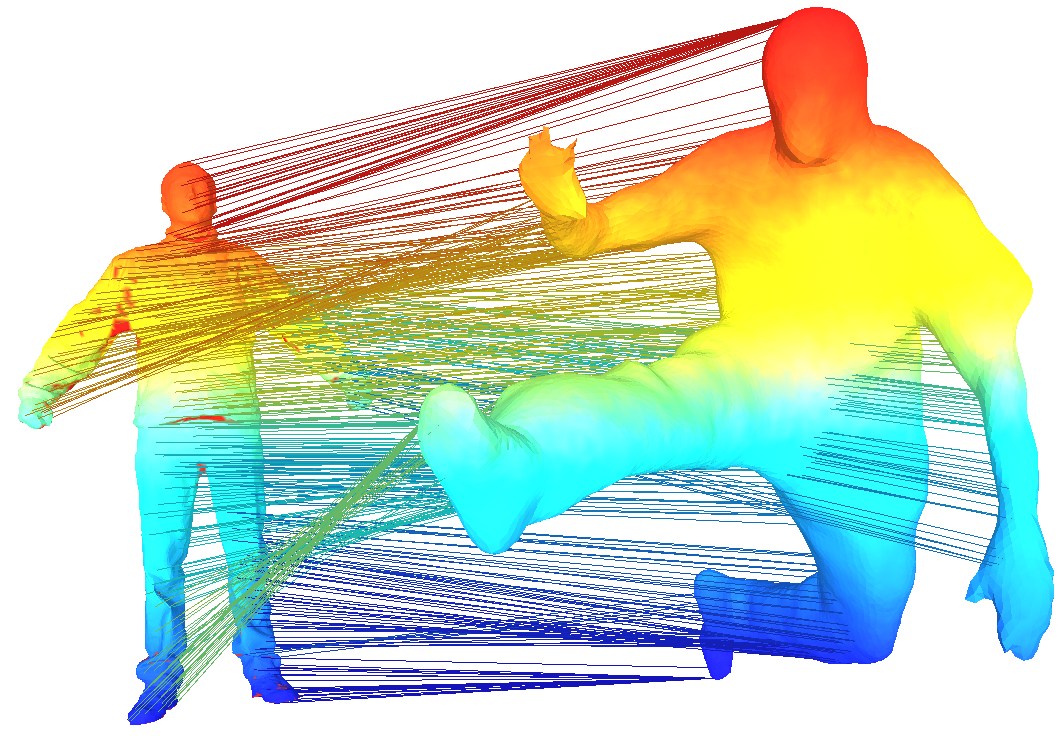
\includegraphics[width=7.0cm]{matching2.png} 
\end{center}

The typical relevant statistics include the number of detected
interest points in the two images, the number of initial and accepted
correspondences, and the mean and standard deviations of the
dissimilarity measure for the accepted matches.
\medskip

For your report, you may conclude what patch size and matching
acceptance criterion you found that gives the best results. Also, you 
may consider if some image patch normalisation could improve the
robustness of the feature matching.
\medskip


At the Absalon course page you may find 3 images
\verb|img001_diffuse|, \\ 
\verb|img002_diffuse| and \verb|img009_diffuse| all showing the same
object from slightly different view angles. Also, you will find smaller
gray scale versions of these images. We recommend that you work on the
latter images. The images are taken from the DTU robot data set
\url{http://roboimagedata.imm.dtu.dk/}.
\medskip

As part of the assignment you should first detect and match interest
points in the images \verb|img001_diffuse| and
\verb|img002_diffuse|.  Next, you should repeat the experiment by
matching \verb|img001_diffuse| with \verb|img009_diffuse|.  Explain
why your performance on this pair of images changes.

\end{document}
